% This is samplepaper.tex, a sample chapter demonstrating the
% LLNCS macro package for Springer Computer Science proceedings;
% Version 2.20 of 2017/10/04
%
\documentclass[runningheads]{llncs}
%
\usepackage{graphicx}
\graphicspath{{images/}}
% Used for displaying a sample figure. If possible, figure files should
% be included in EPS format.
\usepackage{amsmath}
\usepackage[hyphens, spaces]{url}
% If you use the hyperref package, please uncomment the following line
% to display URLs in blue roman font according to Springer's eBook style:
\usepackage{hyperref}
\renewcommand\UrlFont{\color{blue}\rmfamily}
\usepackage[linesnumbered, ruled]{algorithm2e}
\usepackage{mathtools} % for coloneqq
\usepackage{subfig}
\usepackage{booktabs}

\DeclareMathOperator*{\argmin}{arg\,min}

\begin{document}
%
\title{An efficient new static scheduling heuristic for accelerated architectures\thanks{Supported by the Engineering and Physical Sciences Research Council (EPSRC).}}
%
%\titlerunning{Abbreviated paper title}
% If the paper title is too long for the running head, you can set
% an abbreviated paper title here
%
\author{Thomas McSweeney\inst{1}\orcidID{0000-0001-9866-2229} \and Neil Walton\inst{1}\orcidID{0000-0002-5241-9765} \and Mawussi Zounon\inst{1, 2}\orcidID{0000-0002-6955-1500} }
%
\authorrunning{T. McSweeney et al.}
% First names are abbreviated in the running head.
% If there are more than two authors, 'et al.' is used.
%
\institute{University of Manchester, Manchester, UK \\
	\email{thomas.mcsweeney@postgrad.manchester.ac.uk} \and The Numerical Algorithms Group (NAG), Manchester, UK}

%
\maketitle              % typeset the header of the contribution
%
\begin{abstract}

Heterogeneous architectures that use {\em Graphics Processing Units} (GPUs) for general computations, in addition to multicore CPUs, are increasingly common in high-performance computing. However many of the existing methods for scheduling precedence-constrained tasks on such platforms were intended for more diversely heterogeneous clusters, such as the classic {\em Heterogeneous Earliest Finish Time} (HEFT) heuristic. We propose a new static scheduling heuristic called {\em Heterogeneous Optimistic Finish Time} (HOFT) which exploits the binary heterogeneity of accelerated platforms. Through extensive experimentation with custom software for simulating task scheduling problems on user-defined CPU-GPU platforms, we show that HOFT can obtain schedules at least $5\%$ shorter than HEFT's for medium-to-large numerical linear algebra application task graphs and around $3\%$ shorter on average for a large collection of randomly-generated graphs.   


\keywords{High-performance computing \and GPU computing \and Scheduling \and Precedence constraints \and Directed acyclic graphs.}
\end{abstract}


\section{Introduction}
\label{sect.intro}

Modern {\em High-Performance Computing} (HPC) machines typically comprise hundreds or even thousands of networked nodes. These nodes are increasingly likely to be {\em heterogeneous}, hosting one or more powerful accelerators---usually GPUs---in addition to multicore CPUs. For example, Summit, which currently heads the Top500\footnote{\href{https://www.top500.org/}{{\tt \small https://www.top500.org/}}} list of the world's fastest supercomputers, comprises over $4000$ nodes, each with two 22-core IBM Power9 CPUs and six NVIDIA Tesla V100 GPUs. 

Task-based parallel programming is a paradigm that aims to harness this processor heterogeneity. Here a program is described as a collection of {\em tasks}---logically discrete atomic units of work---with {\em precedence constraints} that define the order in which they can be executed. This can be expressed in the form of a graph, where each vertex represents a task and edges the precedence constraints between them. We are interested only in the case when such task graphs are {\em Directed Acyclic Graphs} (DAGs)---directed and without any cycles.  

The immediate question is, how do we find the optimal way to assign the tasks to a set of heterogeneous processing resources while still respecting the precedence constraints? In other words, what {\em schedule} should we follow? This DAG scheduling problem is known to be NP-complete, even for homogeneous processors \cite{topcuoglu2002performance}, so typically we must rely on heuristic algorithms that give us reasonably good solutions in a reasonable time.

A fundamental distinction is made between {\em static} and {\em dynamic} scheduling. Static schedules are fixed before execution based on the information available at that time, whereas dynamic schedules are determined during runtime. There are generic advantages and disadvantages to both: static scheduling makes greater use of the data so is superior when it is sufficiently accurate, whereas dynamic scheduling uses more recent data. In practice task scheduling is usually handled by a {\em runtime system}, such as OmpSs \cite{duran2011ompss}, PaRSEC \cite{bosilca2013parsec}, or StarPU \cite{augonnet2011starpu}. Most such systems use previous execution traces to predict task execution and data transfer times at runtime. On a single machine the latter is tricky because of shared buses and the possibility of asynchronous data transfers. Hence at present dynamic scheduling is typically preferred. However static schedules can be surprisingly robust, even when estimates are poor \cite{agullo2016}. Furthermore, robustness can be improved using timing distribution information \cite{ZHENG20131673}. In addition, superior performance can be achieved in dynamic environments by modifying an existing static schedule, rather than computing a new one from scratch \cite{agullo2016}. 

In this paper we therefore focus on the problem of finding good static schedules for multicore and GPU platforms. To facilitate this investigation, we developed an open-source software simulator which allows users to simulate the static scheduling of arbitrary task DAGs on arbitrary CPU-GPU platforms, without worrying about the time or energy usage constraints imposed by real systems.   
% we therefore focus on... "with the understanding that these can be used as a basis for better dynamic schedules in practice."

The popular HEFT scheduling heuristic comprises two phases: a {\em task prioritization} phase in which the order tasks are to be scheduled is determined and a {\em processor selection} phase in which they are actually assigned to the processing resources. In this article we introduce HOFT, which follows the HEFT framework but modifies both phases in order to exploit accelerated architectures in particular, without significantly increasing the complexity of the algorithm. HOFT works by first computing a table of {\em optimistic} estimates of the earliest possible times all tasks can be completed on both processor types and using this to guide both phases. Simulations with real and randomly-generated DAGs on both single and multiple GPU target platforms suggest that HOFT is always at least competitive with HEFT and frequently superior.     
% Given the ubiquity of accelerated platforms in both HPC and beyond, it is vital that existing scheduling algorithms such as HEFT are optimized to reflect this.  

Explicitly, the two main contributions of this paper are:
\begin{enumerate}	
	\item A new static scheduling heuristic that is optimized specifically for accelerated heterogeneous architectures;
	\item Open-source simulation software that allows researchers to implement and evaluate their own scheduling algorithms for user-defined CPU-GPU platforms in a fast and reproducible manner.
\end{enumerate} 
The remainder of this paper is structured as follows. In Section \ref{sect.lit_review} we summarize the relevant existing literature. Then in Section \ref{sect.simulator} we explicitly define the simulation model we use to study the static task scheduling problem. We describe HEFT in detail in Section \ref{sect.HEFT}, including also benchmarking results with our simulation model and a minor modification to the algorithm that we found performs well. In Section \ref{sect.hoft} we describe our new HOFT heuristic, before detailing the numerical experiments that we undertook to evaluate its performance in Section \ref{sect.results}. Finally in Section \ref{sect.conclusion} we state our conclusions from this investigation and outline future work that we believe may be useful.
 
\section{Related work}
\label{sect.lit_review}

Broadly, static scheduling methods can be divided into three categories: {\em mathematical programming}, {\em guided-random search} and {\em heuristics}. The first is based on formulating the scheduling problem as a mathematical program; see, for example, Kumar's constraint programming formulation in \cite{kumar:tel-01538516}. However solving these is usually so expensive that they are restricted to small task graphs. Guided-random search is a term used for any method that generates a large population of potential schedules and then selects the best among them. Typically these are more general optimization schemes such as genetic algorithms which are refined for the task scheduling problem. As a rule, such methods tend to find very high-quality schedules but take a long time to do so \cite{BRAUN2001810}. 
%for example, a comparison by Braun et al. found that genetic algorithms usually obtained superior schedules to all other alternatives considered but were up to 300 times as expensive (then the citation).

Heuristics are the most popular approach in practice as they are often competitive with the alternatives and considerably faster. In turn {\em listing} heuristics are the most popular kind. They follow a two-phase structure: an ordered list of all tasks is first constructed (task prioritization) and they are then scheduled in this order according to some rule (processor selection). HEFT is the most prominent example: all tasks are prioritized according to their {\em upward rank} and then scheduled on the processor expected to complete their execution at the earliest time; a fuller description is given in Section \ref{sect.HEFT}. Canon et al. \cite{canon2008comparative} compared twenty different task scheduling heuristics and found that HEFT was almost always among the best in terms of both schedule makespan and robustness.

%There are in turn three occasionally overlapping types. {\em Clustering} heuristics work by first grouping all tasks in the DAG and then scheduling each cluster to a single processing resource, with the goal of reducing communication costs \cite{topcuoglu2002performance}. The drawback tends to be that the clustering step is expensive. {\em Duplication-based} heuristics also attempt to reduce communication costs, by ensuring that communicating tasks are scheduled on the same resource even if this requires them to be duplicated---i.e., the same task may be redundantly scheduled in more than one place \cite{duplication}. They can often be superior to alternatives in terms of schedule quality \cite{hcpfd} but they generally also have very high time-complexity bounds \cite{topcuoglu2002performance} since controlling the amount of duplication is tricky: too much can lead to the system becoming clogged, with duplicated tasks obstructing the optimal scheduling of others. 

Many modifications of HEFT have been proposed in the literature, such as HEFT {\em with lookahead} from Bittencourt, Sakellariou and Madeira \cite{bittencourt10}, which has the same task prioritization phase but schedules all tasks on the resources estimated to minimize the completion time of their {\em children}. This has the effect of increasing the time complexity of the algorithm so, in an attempt to incorporate a degree of lookahead into the HEFT framework without increasing the cost, Arabnejad and Barbosa proposed {\em Predict Earliest Finish Time} (PEFT) \cite{arabnejad14}. The main innovation is that rather than just minimizing the completion time of a task during processor selection, we also try to minimize an {\em optimistic} estimate of the time it will take to execute the remaining unscheduled tasks in the DAG. % Conceptually, our new HOFT heuristic is similar to PEFT but also differs in several key aspects. 

Like the majority of existing methods for static DAG scheduling in heterogeneous computing, HEFT was originally intended for clusters with diverse nodes. At least one extension specifically targeting accelerated architectures has been proposed before, namely HEFT-NC ({\em No Cross}) from Shetti, Fahmy and Bretschneider \cite{shetti2013optimization}, but our new HOFT heuristic differs from this in both the task prioritization and processor selection phases of the algorithm.
% HOFT and HEFT-NC can be viewed as similar but HOFT uses ratio of OFT values instead of execution times to rank tasks as this incorporates information from the rest of the DAG, not just the current task. Processor selection phase of HOFT uses OFT table for lookahead to restrict what SFB call "crossover".  

%Agullo et al. \cite{agullo2016} considered static scheduling for individual machines with multicore CPUs and GPUs. After extensive experimentation on real systems they concluded that static schedules can be stable even when the estimates used to compute them are inaccurate. Furthermore, they found that incorporating static analysis into dynamic schedules often improved their performance. 



\section{Simulation model}
\label{sect.simulator}

In this paper we use a simulation model to study the static task scheduling problem for multicore and GPU. This simulator follows the mathematical model described in Section \ref{subsect.mathematical_model} and therefore facilitates the evaluation of scheduling algorithms for idealized CPU-GPU platforms. The advantage of this approach is that it allows us to compare multiple algorithms and determine how intrinsically well-suited they are for accelerated architectures. Although this model may not capture the full range of real-world behavior, we gathered data from a single heterogeneous node of a local computing cluster to guide its development and retain the most salient features. This node comprises four octacore Intel (Skylake) Xeon Gold 6130 CPUs running at 2.10GHz with 192GB RAM and four Nvidia V100-SXM2-16GB (Volta) GPUs, each with 16GB GPU global memory, 5120 CUDA Cores and NVLink interconnect. We used {\em Basic Linear Algebra Subroutine} (BLAS) \cite{Dongarra:1990:SLB:77626.79170} and {\em Linear Algebra PACKage} (LAPACK) \cite{laug} kernels for benchmarking as they are widely-used in scientific computing applications. 

The simulator is implemented in {\tt Python} and the complete source code is available on Github\footnote{\href{https://github.com/mcsweeney90/heterogeneous_optimistic_finish_time}{{\tt \small https://github.com/mcsweeney90/heterogeneous\_optimistic\_finish\_time}}}. All code used to generate results presented in this paper is available in the folder {\tt simulator/scripts} so interested researchers may repeat our experiments for themselves. In addition, users may make modifications to the simulator that they believe will more accurately reflect their own target environment. 


\subsection{Mathematical model}
\label{subsect.mathematical_model}

The simulator software implements the following mathematical model of the problem. Suppose we have a task DAG $G$ consisting of $n$ tasks and $e$ edges that we wish to execute on a target platform $H$ comprising $P$ processing resources of two types, $P_C$ CPU resources and $P - P_C = P_G$ GPU resources. In keeping with much of the related literature and based on current programming practices, we consider CPU cores individually but regard entire GPUs as discrete \cite{agullo2016}. For example, a node comprising 4 GPUs and 4 octacore CPUs would be viewed as 4 GPU resources and $4 \times 8 = 32$ CPU resources.   

We assume that all tasks $t_1, \dots, t_n$ are atomic and cannot be divided across multiple resources or aggregated to form larger tasks. Further, all resources can only execute a single task at any one time and can in principle execute all tasks, albeit with different processing times. Given the increasing versatility of modern GPUs and the parallelism of modern CPUs, the latter is a much less restrictive assumption than it once may have been. 

In our experiments, we found that the spread of kernel processing times was usually tight, with the standard deviation often being two orders of magnitude smaller than the mean. Thus we assume that all task execution times on all processing resources of a single type are identical. In particular, this means that each task has only two possible {\em computation costs}: a CPU execution time $w_C(t_i)$ and a GPU execution time $w_G(t_i)$. When necessary, we denote by $w_{im}$ the processing time of task $t_i$ on the specific resource $p_m$.

The {\em communication cost} between task $t_i$ and its child $t_j$ is the length of time between when execution of $t_i$ is complete and execution of $t_j$ can begin, including all relevant latency and data transfer times. Since this depends on where each task is executed, we view this as a function $c_{ij}(p_m, p_n)$. We assume that the communication cost is always zero when $m = n$ and that there are only four possible communication costs between tasks $t_i$ and $t_j$ when this isn't the case: $c_{ij}(C, C)$, from a CPU to a different CPU; $c_{ij}(C, G)$, from CPU to GPU; $c_{ij}(G, C)$, from GPU to CPU; and $c_{ij}(G, G)$ from GPU to a different GPU.  
% Of course, these assumptions are not representative of all possible CPU-GPU memory architectures but are intended to be reasonable for a typical heterogeneous HPC node today. 

A {\em schedule} is a mapping from tasks to processing resources, as well as the precise time at which their execution should begin. Our goal is to find a schedule which minimizes the {\em makespan} of the task graph, the total execution time of the application it represents. A task with no successors is called an {\em exit} task. Once all tasks have been scheduled, the makespan is easily computed as the earliest time all exit tasks will be completed. Note that although we assume that all costs represent time, they could be anything else we wish to minimize, such as energy consumption, so long as this is done consistently. We do not however consider the multi-objective optimization problem of trading off two or more different cost types here. 



\subsection{Testing environments}
\label{subsect.testing_environment}

In the numerical experiments described later in this article, we consider two simulated target platforms: {\em Single GPU}, comprising 1 GPU and 1 octacore CPU, and {\em Multiple GPU}, comprising 4 GPUs and 4 octacore CPUs. The latter represents the node we used to guide the development of our simulator and the former is considered in order to study how the number of GPUs affects performance. We follow the convention that a CPU core is dedicated to managing each of the GPUs \cite{augonnet2011starpu}, so these two platforms are actually assumed to comprise 7 CPU and 1 GPU resources, and 28 CPU and 4 GPU resources, respectively. Based on our exploratory experiments, we make two further assumptions. First, since communication costs between CPU resources were negligible relative to all other combinations, we assume they are zero---i.e., $c_{ij}(C, C) = 0, \forall i, j$. Second, because CPU-GPU communication costs were very similar to the corresponding GPU-CPU and GPU-GPU costs, we take them to be identical---i.e., $c_{ij}(C, G) = c_{ij}(G, C) = c_{ij}(G, G), \forall i, j$. These assumptions will obviously not be representative of all possible architectures but the simulator software allows users to repeat our experiments for more accurate representations of their own target platforms if they wish. 

We consider the scheduling of two different sets of DAGs. The first consists of ten DAGs comprising between $35$ and $22,100$ tasks which correspond to the {\em Cholesky factorization} of $N \times N$ tiled matrices, where $N = 5, 10, 15, \dots, 50$. In particular, the DAGs are based on a common implementation of Cholesky factorization for tiled matrices which uses {\tt GEMM} (matrix multiplication), {\tt SYRK} (symmetric rank-$k$ update) and {\tt TRSM} (triangular solve) BLAS kernels, as well as the {\tt POTRF} (Cholesky factorization) LAPACK routine \cite{Dongarra:1990:SLB:77626.79170}. All task CPU/GPU processing times are means of 1000 real timings of that task kernel. Likewise, communication costs are sample means of real communication timings between the relevant task and resource types. All numerical experiments were performed for tile sizes $128$ and $1024$; which was used will always be specified where results are presented. Those sizes were chosen as they roughly mark the upper and lower limits of tile sizes typically used for CPU-GPU platforms.

The standard way to quantify the relative amount of communication and computation represented by a task graph is the {\em Computation-to-Communication Ratio} (CCR), the mean computation cost of the DAG divided by the mean communication cost. For the Cholesky DAGs, the CCR was about 1 for tile size 128 and about 18 for tile size 1024, with minor variation depending on the total number of tasks in the DAG. 
% CCR $\coloneqq n \sum_{i, j}\overline{c_{ij}}  / e\sum_{i} \overline{w_i}$ - but haven't defined mean computation and communication costs yet...

We constructed a set of randomly-generated DAGs with a wide range of CCRs, based on the topologies of the 180 DAGs with 1002 tasks from the {\em Standard Task Graph} (STG) set \cite{Tobita2002}. Following the approach in \cite{canon2018}, we selected GPU execution times for all tasks uniformly at random from $[1, 100]$ and computed the corresponding CPU times by multiplying by a random variable from a Gamma distribution. To consider a variety of potential applications, for each DAG we made two copies: {\em low acceleration}, for which the mean and standard deviation of the Gamma distribution was defined to be 5, and {\em high acceleration}, for which both were taken to be $50$ instead. These values roughly correspond to what we observed in our benchmarking of BLAS and LAPACK kernels with tile sizes $128$ and $1024$, respectively. Finally, for both parameter regimes, we made three copies of each DAG and randomly generated communication costs such that the CCR fell into each of the intervals $[0, 10]$, $[10, 20]$ and $[20, 50]$. Thus in total the random DAG set contains $180 \times 2 \times 3 = 1080$ DAGs.  
% The idea is that the two different acceleration regimes will also cover other architectures implicitly.



\section{HEFT}
\label{sect.HEFT}

Recall that as a listing scheduler HEFT comprises two phases, an initial {\em task prioritization} phase in which the order all tasks are to be scheduled is determined and a {\em processor selection} phase in which the processing resource each task is to be scheduled on is decided. Here we describe both in order to give a complete description of the HEFT algorithm.  

The {\em critical path} of a DAG is the longest path through it, and is important because it gives a lower bound on the optimal schedule makespan for that DAG. Heuristics for homogeneous platforms often use the {\em upward rank}, the length of the critical path from that task to an exit task, including the task itself \cite{topcuoglu2002performance}, to determine priorities. Computing the critical path is not straightforward for heterogeneous platforms so HEFT extends the idea by using {\em mean} values instead. Intuitively, the task prioritization phase of HEFT can be viewed as an approximate dynamic program applied to a simplified version of the task DAG that uses mean values to set all weights.

More formally, we first define the {\em mean execution cost} of all tasks $t_i$ through
\begin{equation}
\label{eq.avg_comp}
\overline{w_i} \coloneqq \sum_{m = 1}^{P} \frac{w_{im}}{P} = \frac{w_C(t_i) P_C + w_G(t_i) P_G}{P},
\end{equation}  
where the second expression is how $\overline{w_i}$ would be computed under the assumptions of our model. Likewise, the {\em mean communication cost} $\overline{c_{ij}}$ between $t_i$ and $t_j$ is the average of all such costs over all possible combinations of resources,
\begin{align}
\label{eq.avg_comm}
\overline{c_{ij}} = \frac{1}{P^2}\sum_{m, n} c_{ij}(p_m, p_n) = \frac{1}{P^2}\sum_{k, \ell \in \{ C, G \}} A_{k\ell} c_{ij}(k, \ell),
\end{align}
where $A_{CC} = P_C(P_C - 1)$, $A_{CG} = P_C P_G = A_{GC}$, and $A_{GG} = P_G(P_G - 1)$. 
For all tasks $t_i$ in the DAG, we define their upward ranks $rank_u(t_i)$ recursively, starting from the exit task(s), by
\begin{align}
\label{eq.upward_rank}
rank_u(t_i) = \overline{w_i} + \max_{t_j \in Ch(t_i)} (\overline{c_{ij}} + rank_u(t_j)),
\end{align}
where $Ch(t_i)$ is the set of $t_i$'s immediate successors in the DAG. The task prioritization phase then concludes by listing all tasks in decreasing order of upward rank, with ties broken arbitrarily. 

The processor selection phase of HEFT is now straightforward: we move down the list and assign each task to the resource expected to complete its execution at the earliest time. Let $R_{m_i}$ be the earliest time at which the processing resource $p_m$ is actually free to execute task $t_i$, $Pa(t_i)$ be the set of $t_i$'s immediate predecessors in the DAG, and $AFT(t_k)$ be the time when execution of a task $t_k$ is actually completed (which in the static case is known precisely once it has been scheduled). Then the {\em earliest start time} of task $t_i$ on processing resource $p_m$ is computed through
\begin{align}
\label{eq.EST}
EST(t_i, p_m) = \max \bigg\{ R_{m_i}, \max_{t_k \in Pa(t_i)} (AFT(t_k) + c_{ki}(p_k, p_m)) \bigg\}
\end{align}
and the {\em earliest finish time} $EFT(t_i, p_m)$ of task $t_i$ on $p_m$ is given by 
\begin{align}
\label{eq.EFT}
EFT(t_i, p_m) = w_{im} + EST(t_i, p_m).
\end{align}
HEFT follows an {\em insertion-based} policy that allows tasks to be inserted between two that are already scheduled, assuming precedence constraints are still respected, so $R_{m_i}$ may not simply be the latest finish time of all tasks on $p_m$. A complete description of HEFT is given in Algorithm \ref{alg.HEFT}. HEFT has a time complexity of $O(P \cdot e)$. For dense DAGs, the number of edges is proportional to $n^2$, where $n$ is the number of tasks, so the complexity is effectively $O(n^2P)$ \cite{topcuoglu2002performance}. 
\begin{algorithm}	
	
	Set the computation cost of all tasks using \eqref{eq.avg_comp}
	
	Set the communication cost of all edges using \eqref{eq.avg_comm}
	
	Compute $rank_u$ for all tasks according to \eqref{eq.upward_rank}
	
	Sort the tasks into a priority list by non-increasing order of $rank_u$
	
	\For{task in list}
	{	
		
		\For{each resource $p_k$}
		{Compute $EFT(t_i, p_k)$ using \eqref{eq.EST} and \eqref{eq.EFT}}
		
		$p_m \coloneqq \argmin_k(EFT(t_i, p_k))$
		
		Schedule $t_i$ on the resource $p_m$ 
		
	}	
	\caption{HEFT.}
	\label{alg.HEFT}
\end{algorithm} 


\subsection{Benchmarking}
\label{subsect.benchmarking}

Using our simulation model, we investigated the quality of the schedules computed by HEFT for the Cholesky and randomly-generated DAG sets on both the single and multiple GPU target platforms described in Section \ref{sect.simulator}. The metric used for evaluation was the {\em speedup}, the ratio of the {\em minimal serial time} (MST)---the minimum execution time of the DAG on any single resource---to the makespan. Intuitively, speedup tells us how well the schedule exploits the parallelism of the target platform.

Figure \ref{plot.heft_benchmark_cholesky} shows the speedup of HEFT for the Cholesky DAGs with tile size $128$. The most interesting takeaway is the difference between the two platforms. With multiple GPUs the speedup increased uniformly with the number of tasks until a small decline for the very largest DAG, but for a single GPU the speedup stagnated much more quickly. This was due to the GPU being continuously busy and adding little additional value once the DAGs became sufficiently large and more GPUs therefore postponing this effect. Results were broadly similar for Cholesky DAGs with tile size $1024$, with the exception that the speedup values were uniformly smaller, reaching a maximum of just over four for the multiple GPU platform. This was because the GPUs were so much faster for the larger tile size that HEFT made little use of the CPUs and so speedup was almost entirely determined by the number of GPUs available. 
\begin{figure}
	\centering	
	\subfloat[Cholesky.]{\label{plot.heft_benchmark_cholesky}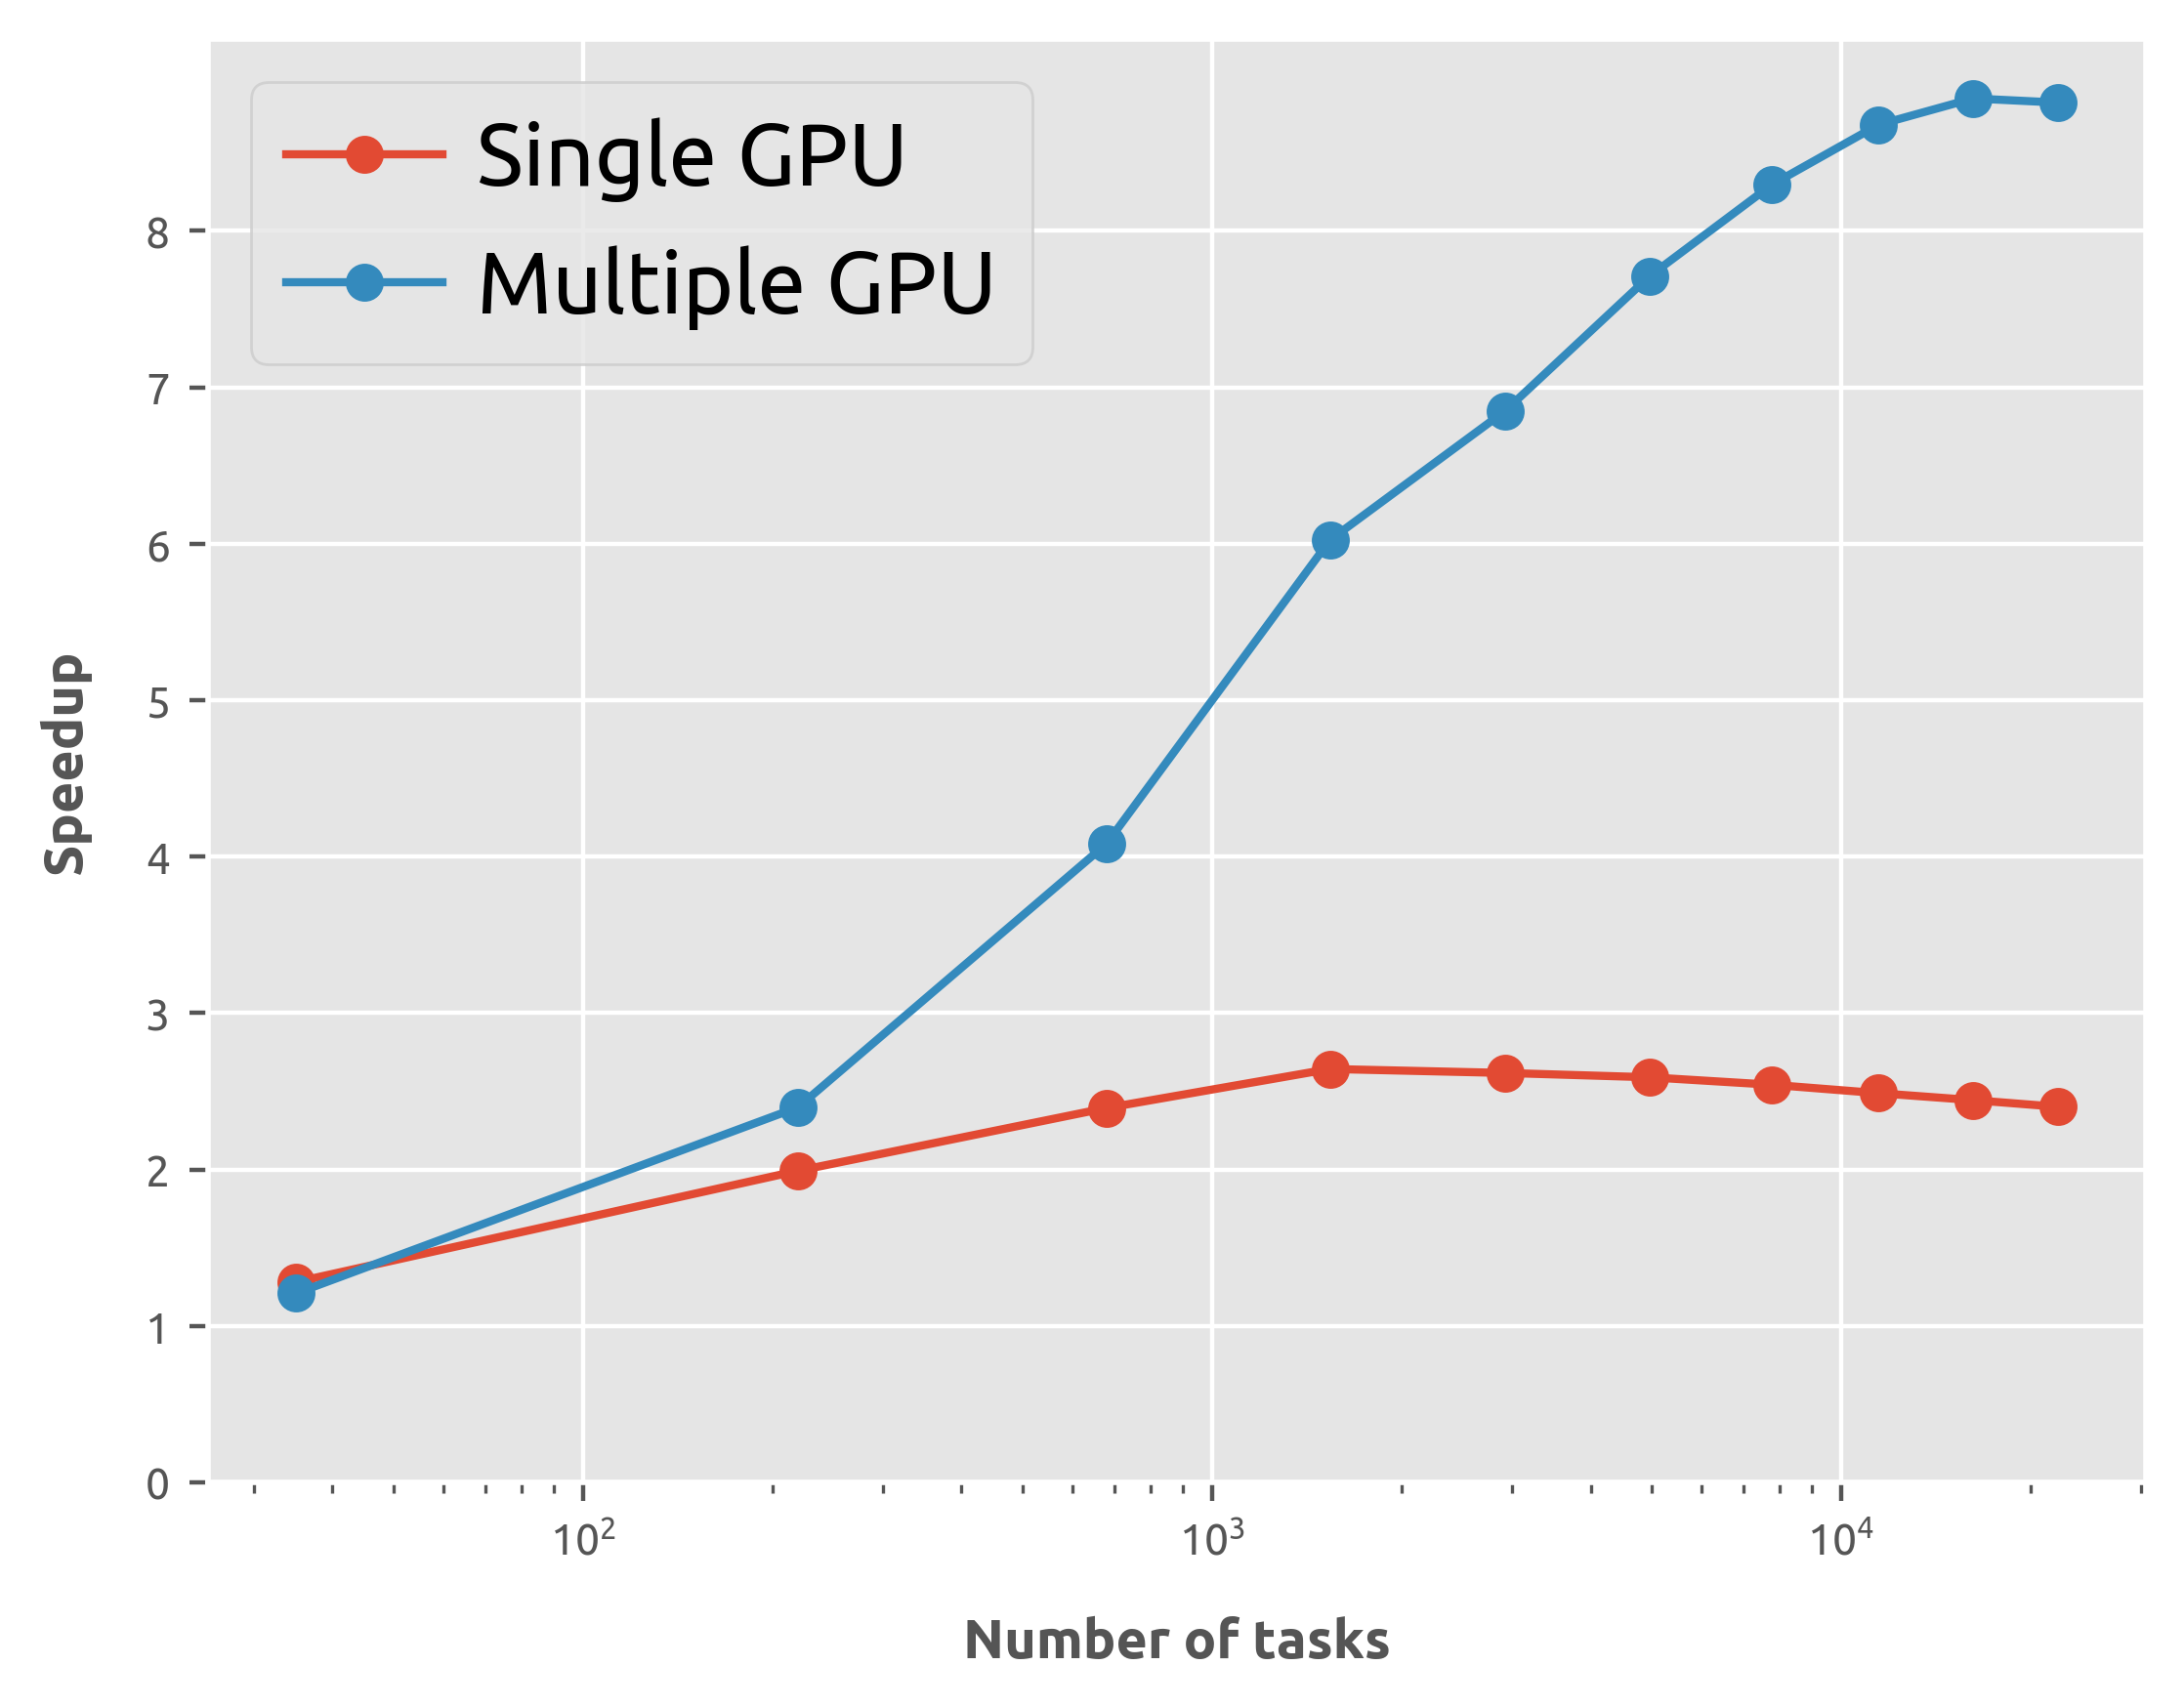
\includegraphics[scale=0.4]{cholesky_nb128_speedups.png}}
	\subfloat[Random.]{\label{plot.heft_benchmark_random}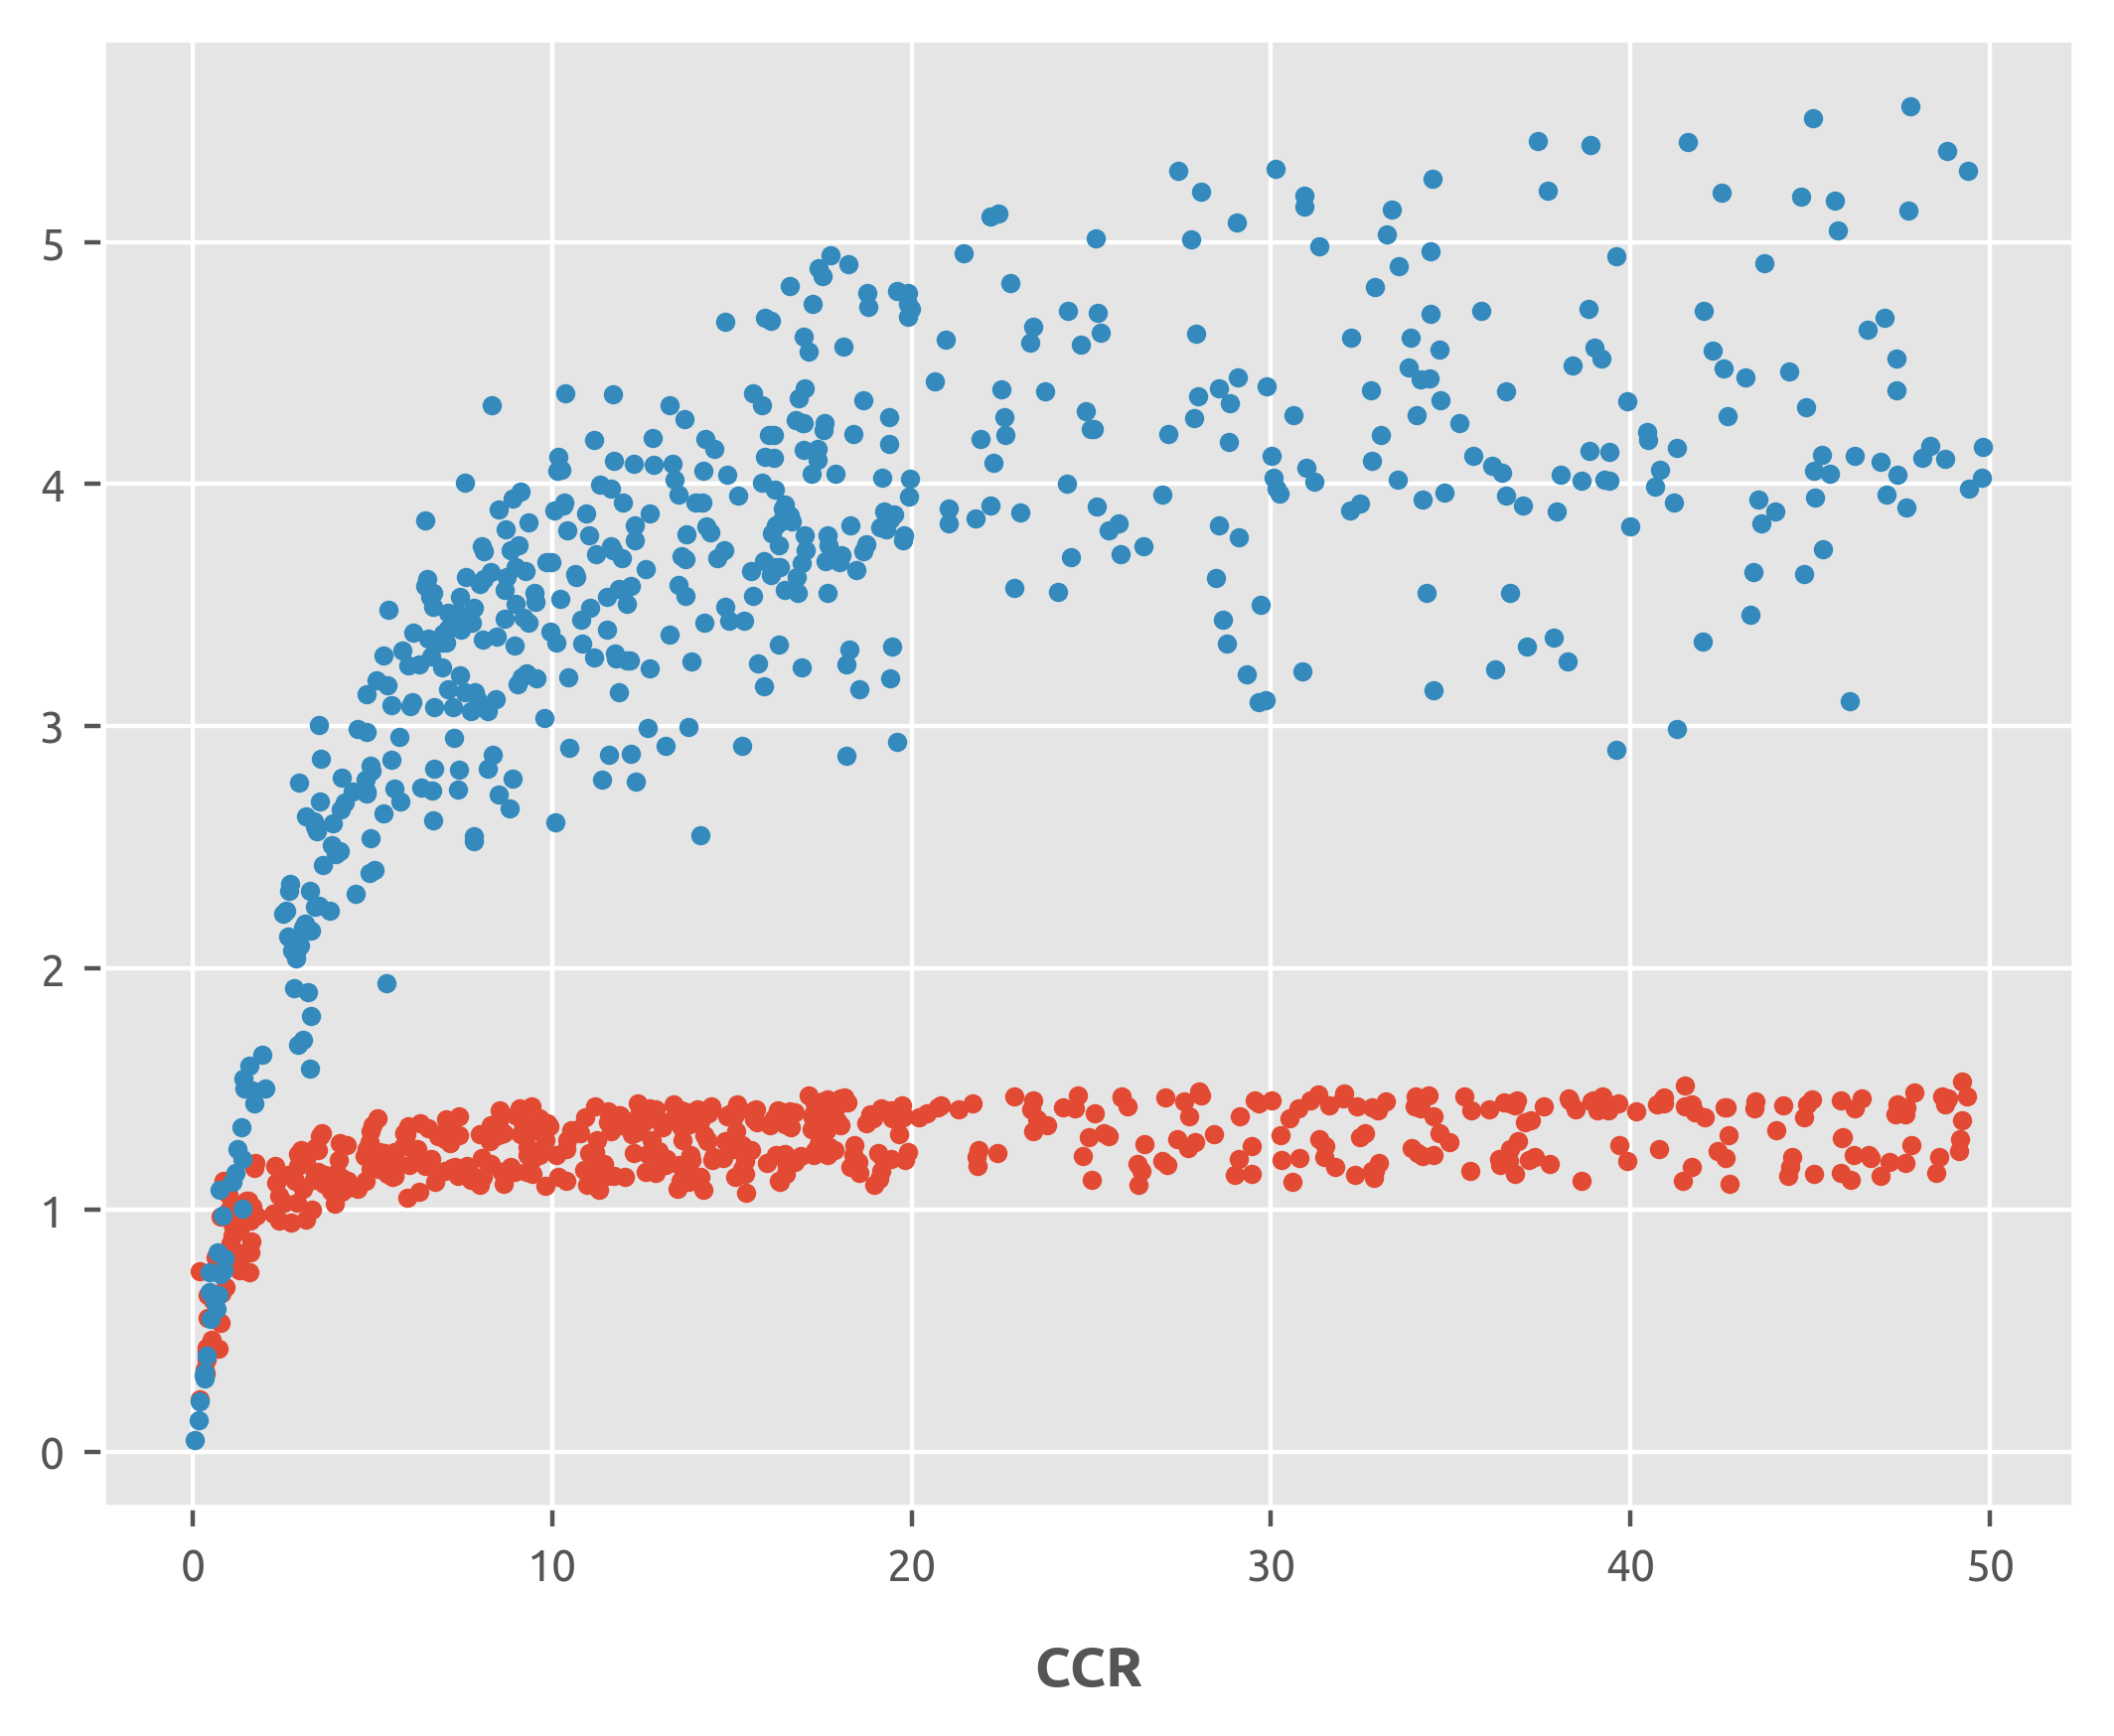
\includegraphics[scale=0.4]{random_speedups_high_acc.png}}
	\caption{Speedup of HEFT for Cholesky (tile size $128$) and random (high acceleration) DAG sets.}	
	\label{plot.heft_benchmark}
\end{figure}

Figure \ref{plot.heft_benchmark_random} shows the speedups for all 540 high acceleration randomly-generated DAGs, ordered by their CCRs; results were broadly similar for the low acceleration DAGs. The speedups for the single GPU platform are much smaller with a narrower spread compared to the other platform, as for the Cholesky DAGs. More surprising is that HEFT sometimes returned a schedule with speedup less than one for DAGs with small CCR values, which we call a {\em failure} since this is obviously unwanted behavior. These failures were due to the greediness of the HEFT processor selection phase, which always schedules a task on the processing resource that minimizes its earliest finish time without considering the communication costs that may later be incurred by doing so. The effect is more pronounced when the CCR is low because the unforeseen communication costs are proportionally larger. 


\subsection{HEFT-WM}
\label{subsect.heft_WM}

The implicit assumption underlying the use of mean values when computing task priorities in HEFT is that the probability of a task being scheduled on a processing resource is identical for all resources. But this is obviously not the case: if a task's GPU execution time is ten times smaller than its CPU execution time then it is considerably more likely to be scheduled on a GPU, even if not precisely ten times so. This suggests that we should weight the mean values according to each task's {\em acceleration ratio} $r_i$, the CPU time divided by the GPU time. In particular, for each task $t_i$ we estimate its computation cost to be
\begin{equation}
\label{eq.avg_comp_wm}
\overline{w_i} = \frac{w_C(t_i) P_C + r_iw_G(t_i) P_G}{P_C + r_iP_G},
\end{equation}  
and for each edge (say, between tasks $t_i$ and $t_j$) the estimated communication cost is
\begin{equation}
\label{eq.avg_comm_wm}
\overline{c_{ij}} = \frac{A_{CC} \cdot c_{ij}(C, C) + A_{CG}\big(r_ic_{ij}(G, C) + r_jc_{ij}(C, G)\big) + r_ir_j A_{GG} \cdot c_{ij}(G, G) }{(r_iP_G + P_C) \cdot (r_jP_G + P_C)}. 
\end{equation}
We call the modified heuristic which follows Algorithm \ref{alg.HEFT} but uses \eqref{eq.avg_comp_wm} instead of \eqref{eq.avg_comp} and \eqref{eq.avg_comm_wm} instead of \eqref{eq.avg_comm} HEFT-WM (for {\em Weighted Mean}). We were unable to find any explicit references to this modification in the literature but given its simplicity we do not think it is a novel idea and suspect it has surely been used before in practice.    


\section{HOFT}
\label{sect.hoft}

If we disregard all resource contention, then we can easily compute the earliest possible time that all tasks can be completed assuming that they are scheduled on either a CPU or GPU resource, which we call the {\em Optimistic Finish Time} (OFT). More specifically, for $p, p' \in \{C, G\}$, we move forward through the DAG and build a table of OFT values by setting $OFT(t_i, p) = w_p(t_i)$, if $t_i$ is an entry task, and recursively computing     
\begin{align}
\label{eq.oft_table}
OFT(t_i, p) &= w_p(t_i) + \max_{t_j \in Pa(t_i)} \bigg \{ \min_{p'} \{ OFT(t_j, p') + \delta_{pp'} c_{ij} (p, p') \}  \bigg \}, 
\end{align}
for all other tasks, where $\delta_{pp'} = 1$ if $p = p'$ and $0$ otherwise. We use the OFT table as the basis for the task prioritization and processor selection phases of a new HEFT-like heuristic optimized for CPU-GPU platforms that we call {\em Heterogeneous Optimistic Finish Time} (HOFT). Note that computing the OFT table does not increase the order of HEFT's time complexity.  


Among several possible ways of using the OFT to compute a complete task prioritization, we found the most effective to be the following. First, define the weights of all tasks to be the ratio of the maximum and minimum OFT values,
\begin{align}
\label{eq.hoft_weights}
\overline{w_i} = \frac{\max\{ OFT(t_i, C), OFT(t_i, G) \}}{\min\{ OFT(t_i, C), OFT(t_i, G) \}}.
\end{align} 
Now assume that all edge weights are zero, $\overline{c_{ij}} \equiv 0, \forall i, j$, and compute the upward rank of all tasks with these values. Upward ranking is used to ensure that all precedence constraints are met. Intuitively, tasks with a strong preference for one resource type---as suggested by a high ratio---should be scheduled first. 

We also propose a new processor selection phase which proceeds as follows. Working down the priority list, each task $t_i$ is scheduled on the processing resource $p_{m}$ with the smallest EFT as in HEFT except when $p_m$ is not also the fastest resource type for that task. In such cases, let $p_f$ be the resource of the fastest type with the minimal EFT and compute 
\begin{align}
\label{eq.sm}
s_m \coloneqq EFT(t_i, p_f) - EFT(t_i, p_m),
\end{align}
the saving that we expect to make by scheduling $t_i$ on $p_m$ rather than $p_f$. Suppose that $p_m$ is of type $T_m \in \{C, G\}$. By assuming that each child task $t_j$ of $t_i$ is scheduled on the type of resource $T_j$ which minimizes its OFT and disregarding the potential need to wait for other parent tasks to complete, we estimate $E(Ch(t_i) | p_m)$, the earliest finish time of all child tasks, given that $t_i$ is scheduled on $p_m$, through
\begin{align}
\label{eq.oft_children}
E(Ch(t_i) | p_m) \coloneqq \max_{t_j \in Ch(t_i)} \Big( EFT(t_i, p_m) + c_{ij}(T_m, T_j) + w_{T_j}(t_j)\Big).
\end{align}
Likewise for $p_f$ we compute $E(Ch(t_i) | p_f)$ and if
\begin{align}
\label{eq.cross_condition}
s_m > E(Ch(t_i) | p_m) - E(Ch(t_i) | p_f)
\end{align}
we schedule task $t_i$ on $p_m$; otherwise, we schedule it on $p_f$. Intuitively, the processor selection always chooses the resource with the smallest EFT unless by doing so we expect to increase the earliest possible time at which all child tasks can be completed.

\begin{algorithm}	
	
	Compute the OFT table for all tasks using \eqref{eq.oft_table}
	
	Set the computation cost of all tasks using \eqref{eq.hoft_weights}
	
	Set the communication cost of all edges to be zero
	
	Compute $rank_u$ for all tasks according to \eqref{eq.upward_rank}
	
	Sort the tasks into a priority list by non-increasing order of $rank_u$
	
	\For{task in list}
	{	
		
		\For{each resource $p_k$}
		{Compute $EFT(t_i, p_k)$ using \eqref{eq.EST} and \eqref{eq.EFT}}	
		
		$p_m \coloneqq \argmin_k(EFT(t_i, p_k))$
		
		\If{$w_{im} \neq \min(w_C(t_i), w_G(t_i))$}{
			
		$p_f \coloneqq \argmin_k\big( EFT(t_i, p_k)| w_{ik} = \min(w_C(t_i), w_G(t_i)) \big)$	
		
		Compute $s_m$ using \eqref{eq.sm}
		
		Compute $E(Ch(t_i) | p_m)$ and $E(Ch(t_i) | p_f)$ using \eqref{eq.oft_children}
		
		\uIf{\eqref{eq.cross_condition} holds}{Schedule $t_i$ on $p_m$}
		\Else{Schedule $t_i$ on $p_f$}			
		}
		
	}	
	\caption{HOFT.}
	\label{alg.HOFT}
\end{algorithm} 

\section{Simulation results}
\label{sect.results}

Figure \ref{plot.hoft_cholesky} shows the reduction in schedule makespan, as a percentage of the HEFT schedule, achieved by HOFT and HEFT-WM for the set of Cholesky DAGs, on both the single and multiple GPU target platforms. The overall trend for the multiple GPU platform is that HOFT improves relative to both HEFT variants as the number of tasks in the DAG grows larger; it is always better than standard HEFT for tile size 1024. For the single GPU platform, HOFT was almost always the best, except for the smallest DAGs and the largest DAG with tile size 128 (for which all three heuristics were almost identical). Interestingly, we found that the processor selection phase of HOFT never actually differed from HEFT's for these DAGs and so the task prioritization phase alone was key. 
\begin{figure}
	\centering	
	\subfloat[Tile size 128.]{\label{plot.hoft_cholesky_nb128}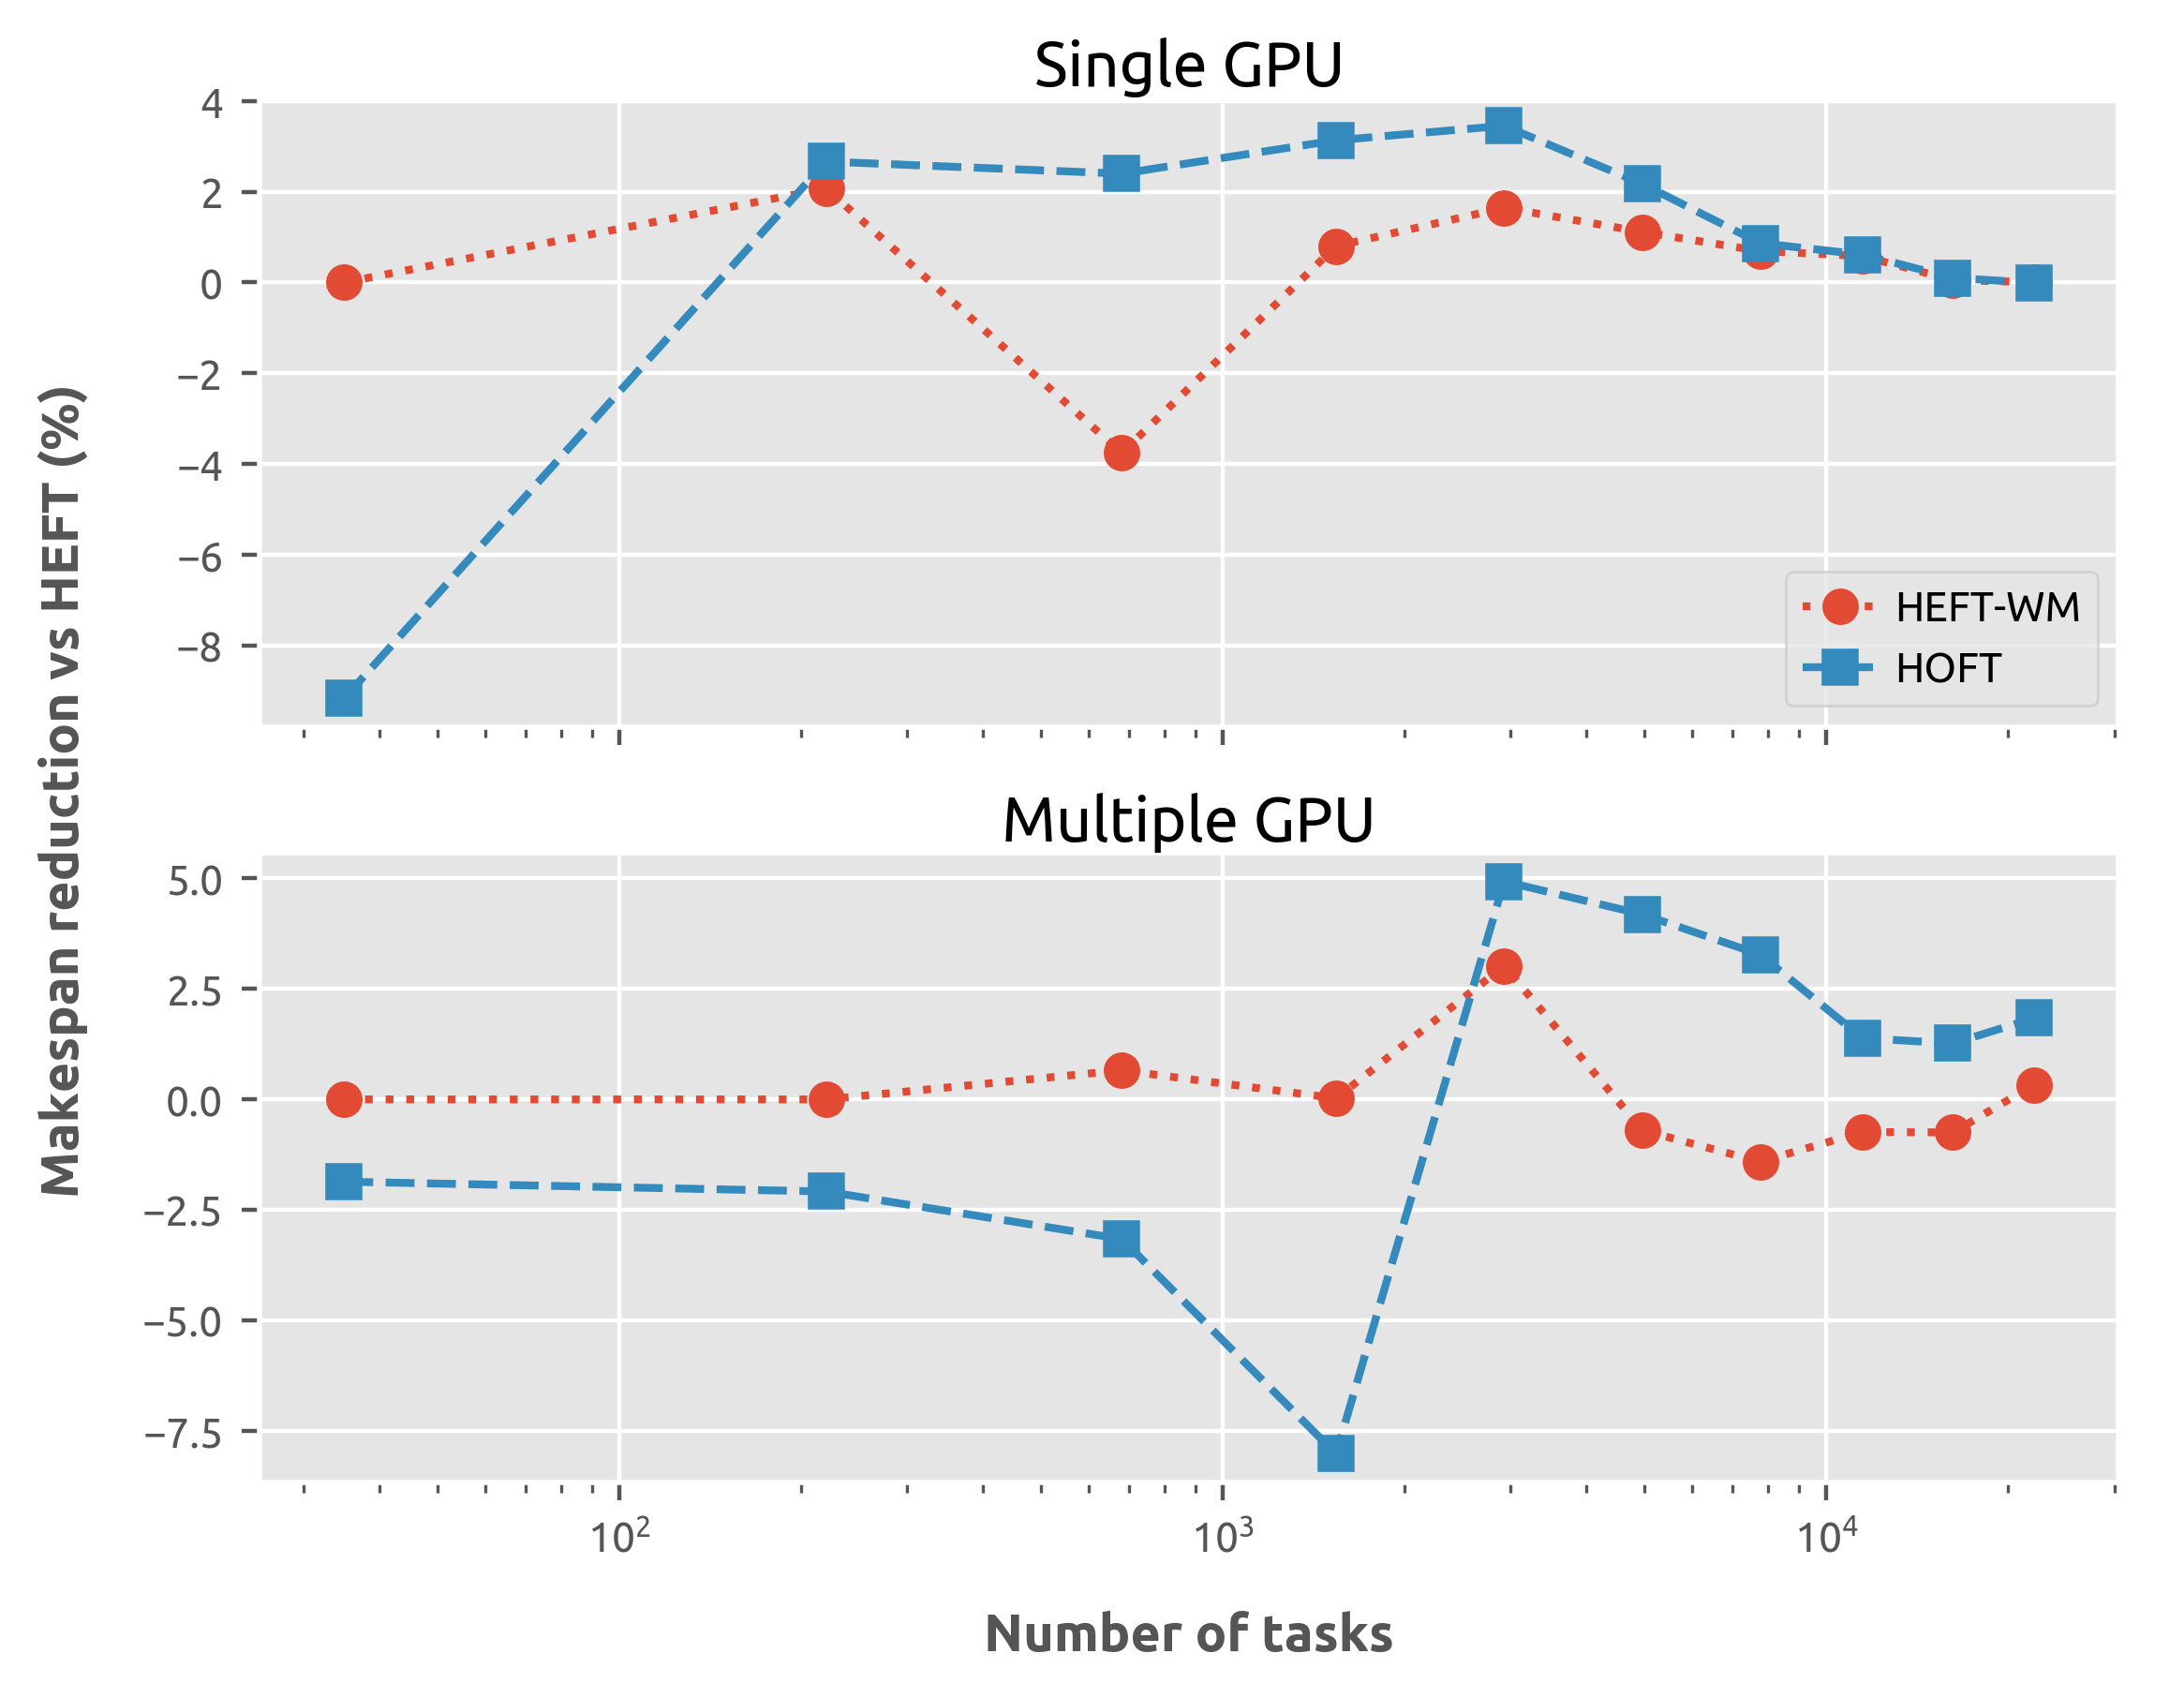
\includegraphics[scale=0.45]{hoft_speedup_cholesky_nb128.png}}
	\subfloat[Tile size 1024.]{\label{plot.hoft_cholesky_nb1024}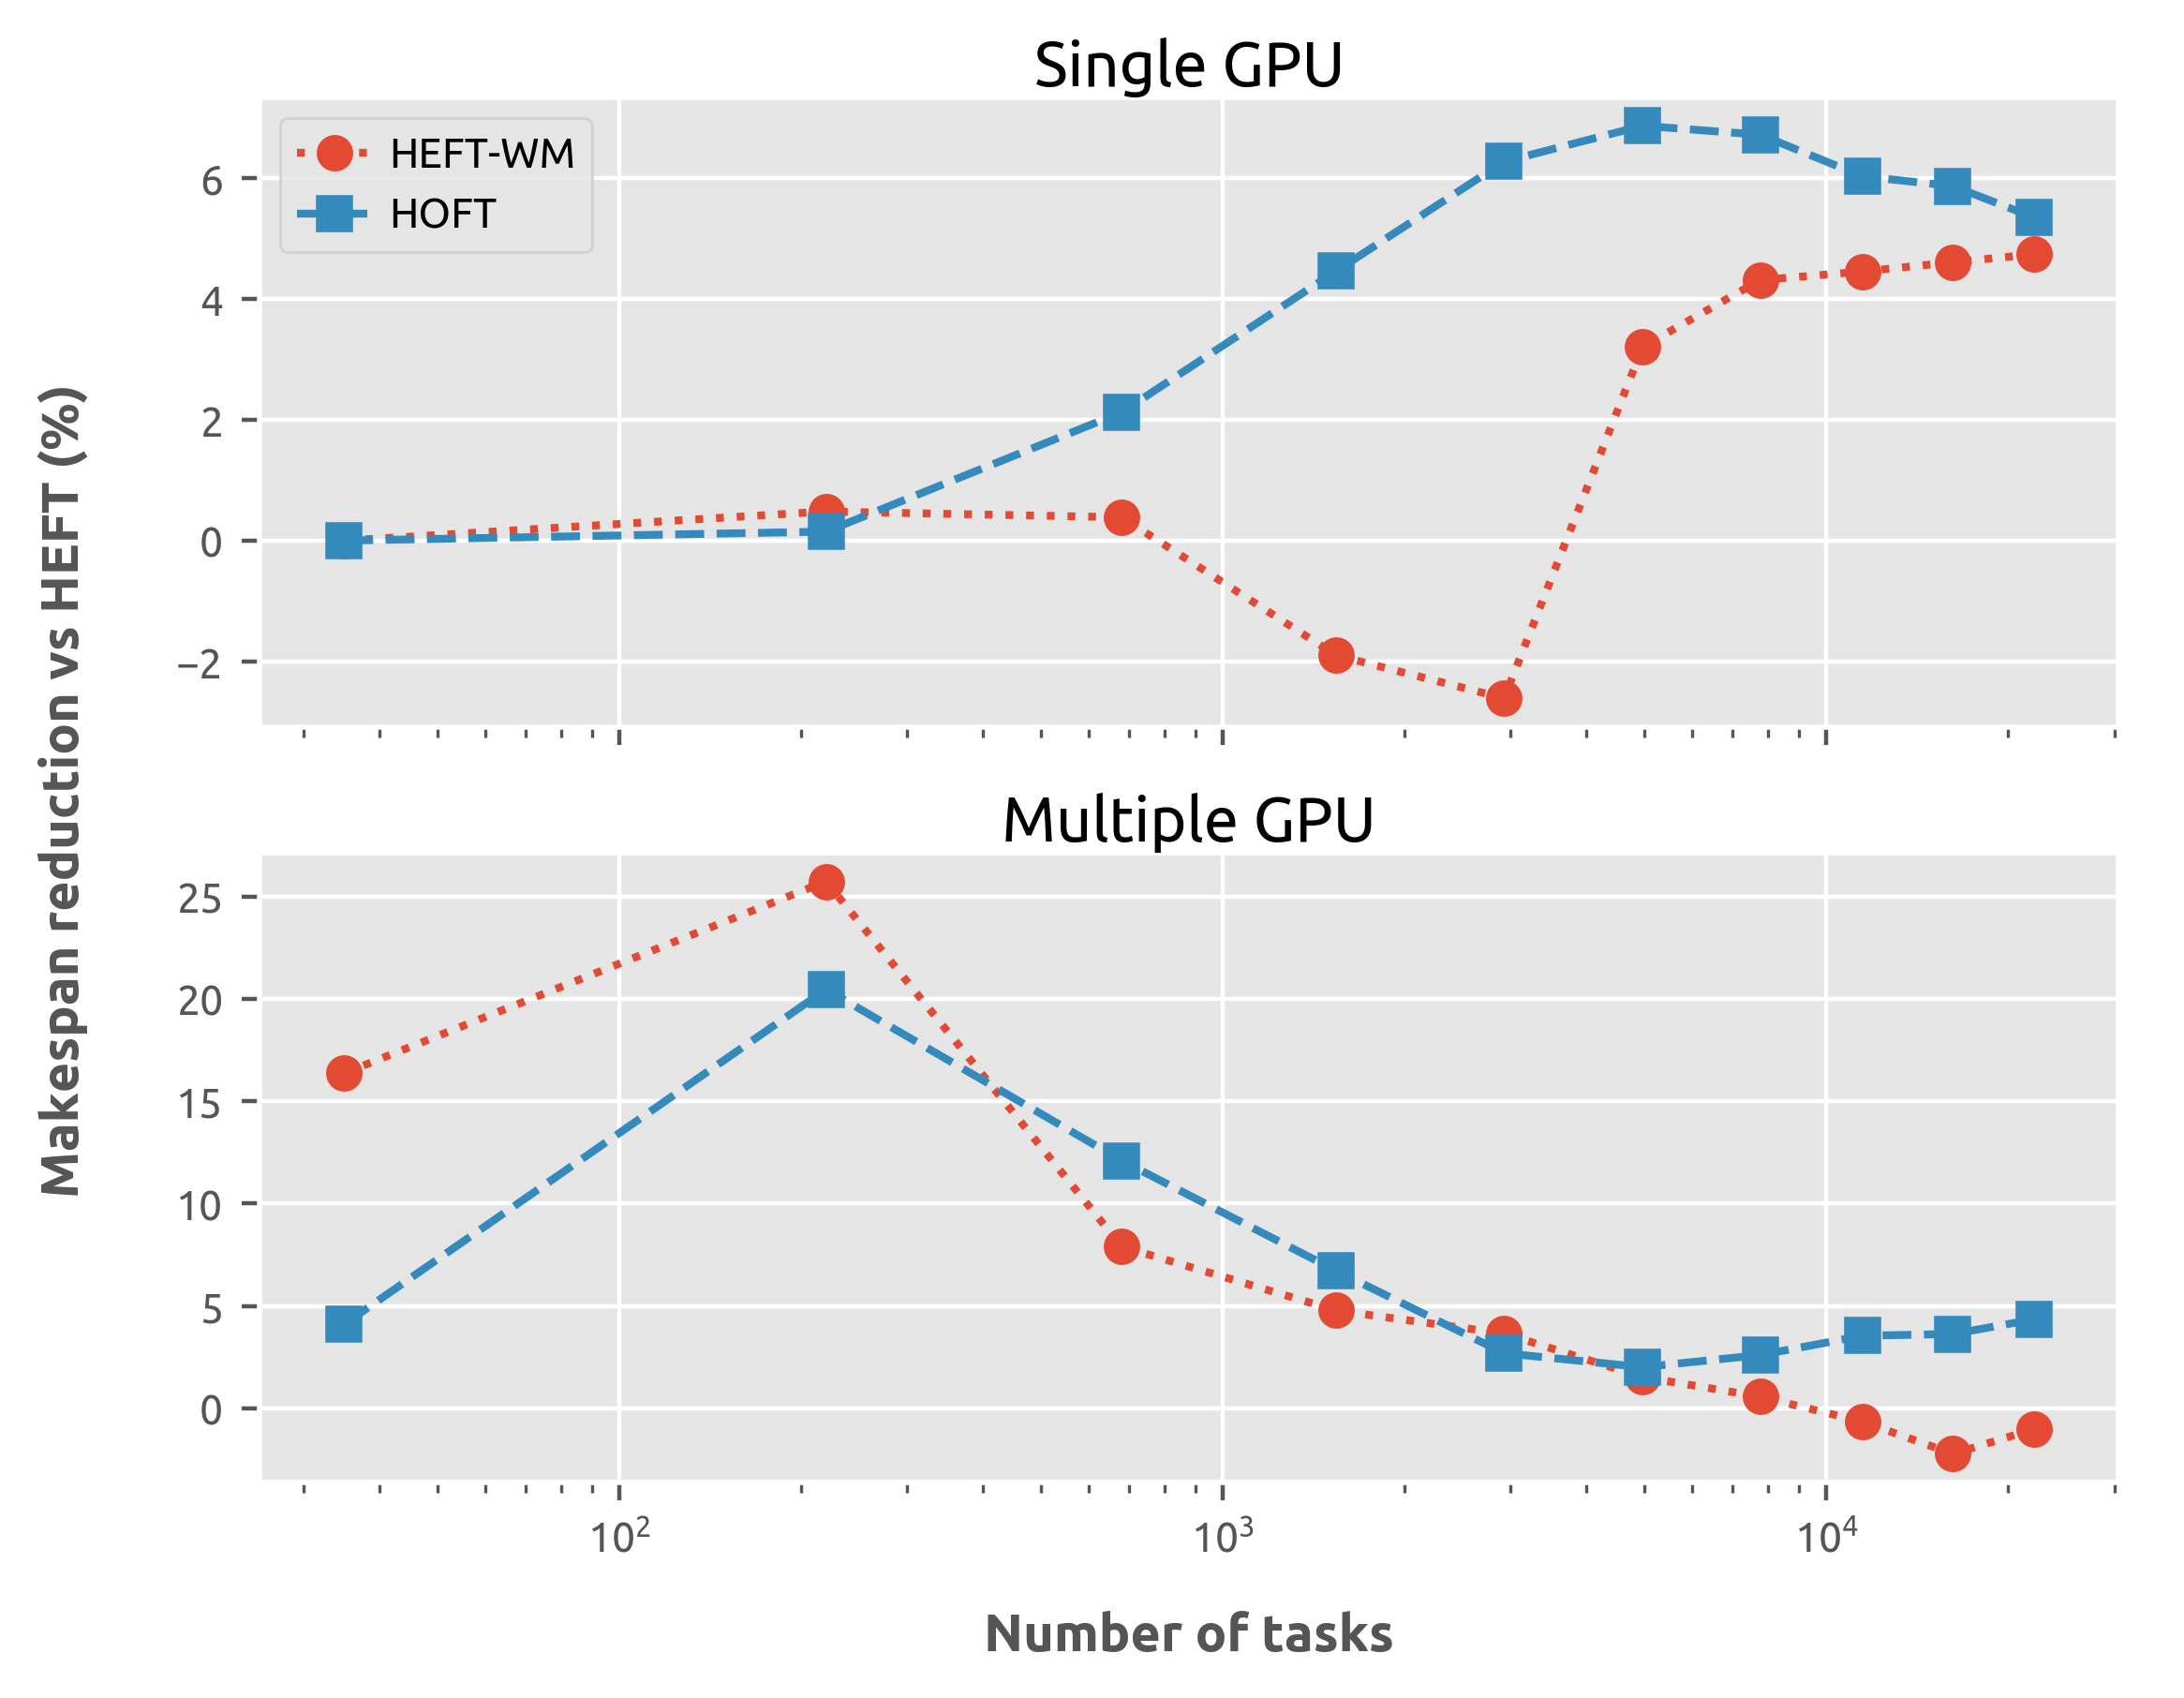
\includegraphics[scale=0.45]{hoft_speedup_cholesky_nb1024.png}}
	\caption{HEFT-WM and HOFT compared to HEFT for Cholesky DAGs.}	
	\label{plot.hoft_cholesky}
\end{figure} 

HOFT achieved smaller makespans than HEFT on average for the set of randomly-generated DAGs, especially for those with high acceleration, but was slightly inferior to HEFT-WM, as can be seen from Table \ref{tb.hoft_random_DAGs}. However also included in the table is HOFT-WM, the heuristic obtained by using the HEFT-WM task prioritization with the HOFT processor selection. HOFT-WM was identical to HEFT-WM for the Cholesky DAGs but improved on both heuristics for the randomly-generated DAG set, suggesting that the HOFT processor selection phase is generally more effective than HEFT's, no matter which task ranking is used. The alternative processor selection also reduced the failure rate for DAGs with very low CCR by about half on the single GPU platform, although it made little difference on the multiple GPU platform.

\begin{table}
	\caption{Makespan reduction vs. HEFT. Shown are both the average percentage reduction ({\em APR}) and the percentage of ($540$) DAGs for which each heuristic improved on the HEFT schedule ({\em Better}).} 
	\begin{center}	
		\begin{tabular}{c c c c c c c c c c c c}
			\toprule
			& \multicolumn{5}{c}{Single GPU} && \multicolumn{5}{c}{Multiple GPU}\\
			\cmidrule{2-6} \cmidrule{8-12}
			& \multicolumn{2}{c}{Low acc.} && \multicolumn{2}{c}{High acc.} && \multicolumn{2}{c}{Low acc.} && \multicolumn{2}{c}{High acc.}\\
			\cmidrule{2-3} \cmidrule{5-6} \cmidrule{8-9} \cmidrule{11-12}
			Heuristic & {\em APR} & {\em Better} && {\em APR} & {\em Better} && {\em APR} & {\em Better} && {\em APR} & {\em Better}\\
			\cmidrule{1-12}
			HEFT-WM & $0.8$ & 74.8 && $2.3$ & 69.6 && $1.6$ & 84.8 && $2.4$ & 79.8\\
			HOFT & $-0.2$ & 50.3 && $3.8$ & 83.1 && $1.4$ & 69.2 && $2.3$ & 76.5\\
			HOFT-WM & $0.8$ & 70.9 && $4.6$ & 76.9 && $1.4$ & 78.1 && $3.7$ & 81.1\\ 
			\bottomrule			
		\end{tabular}
		\label{tb.hoft_random_DAGs}
	\end{center}	
\end{table}


\section{Conclusions}
\label{sect.conclusion}

Overall our simulations suggest that HOFT is often superior to---and always competitive with---both standard HEFT and HEFT-WM for multicore and GPU platforms, especially when task acceleration ratios are high. The processor selection phase in particular appears to be more effective, at least on average, for any task prioritization. It should also be noted that HEFT-WM was almost always superior to the standard algorithm in our simulations, suggesting that it should perhaps be the default in accelerated environments. 

Although the number of failures HOFT recorded for DAGs with low CCRs was slightly smaller than for HEFT, the failure probability was still unacceptably high. Using the lookahead processor selection from \cite{bittencourt10} instead reduced the probability of failure further but it was still nonzero and the additional computational cost was considerable. We investigated cheaper {\em sampling-based} selection phases that consider only a small sample of the child tasks, selected either at random or based on priorities. These did reduce the failure probability in some cases but the improvement was usually minor. Alternatives to lookahead that we intend to consider in future are the duplication \cite{duplication} or aggregation of tasks.

Static schedules for multicore and GPU are most useful in practice as a foundation for superior dynamic schedules \cite{agullo2016}, or when their robustness is reinforced using statistical analysis \cite{ZHENG20131673}. This paper was concerned with computing the initial static schedules; the natural next step is to consider their extension to real---i.e., dynamic---environments. This is often called {\em stochastic} scheduling, since the costs are usually modeled as random variables from some---possibly unknown---distribution. The goal is typically to find methods that bound variation in the schedule makespan, which is notoriously difficult \cite{hagstrom88}. Experimentation with existing stochastic scheduling heuristics, such as {\em Monte Carlo Scheduling} \cite{ZHENG20131673}, suggested to us that the main issue with adapting such methods for multicore and GPU is their cost, which can be much greater than computing the static schedule itself. Hence in future work we intend to investigate cheaper ways to make effective use of static schedules for real platforms.  



%Other things we might consider in future work:
%\begin{itemize}
%	\item How to construct more amenable task DAGs for a given application. For example, in numerical linear algebra applications, we want to know what size the tiles should be (and potentially their shape, whether they should all be uniform, etc).
%	\item Tasks that must be executed by processors of a certain type. 
%	\item Splitting of tasks. For example, a task may be scheduled on a processor and then broken down into subtasks for multiple threads.  
%\end{itemize}  



%
% ---- Bibliography ----
%
% BibTeX users should specify bibliography style 'splncs04'.
% References will then be sorted and formatted in the correct style.
%
 \bibliographystyle{splncs04}
 \bibliography{references}

\end{document}
